% \frame{
%   \frametitle{Exponential Trees\footnote{Andersson, Arne (October 1996)}}
%   \begin{itemize}
%     \item Root has $n^{1/k}$ children, each of which is an exponential tree of size $n^{1-1/k}$, for a fixed constant $k$.
    
%     \medskip
    
%     \item Uses a static data structure lookup within the $n^{1/k}$ children.
%   \end{itemize}
% }


\frame{
  \frametitle{Exponential Trees\footnote{Andersson, Arne (October 1996)}}
  \begin{columns}
    \begin{column}{0.45\textwidth}
    \begin{itemize}
            \item Has niche uses in hash tables 
            
    \medskip
    
            \item Time complexity is a \textit{bit cursed}
        \end{itemize}
    \end{column}
    \begin{column}{0.55\textwidth}
        \begin{center}
         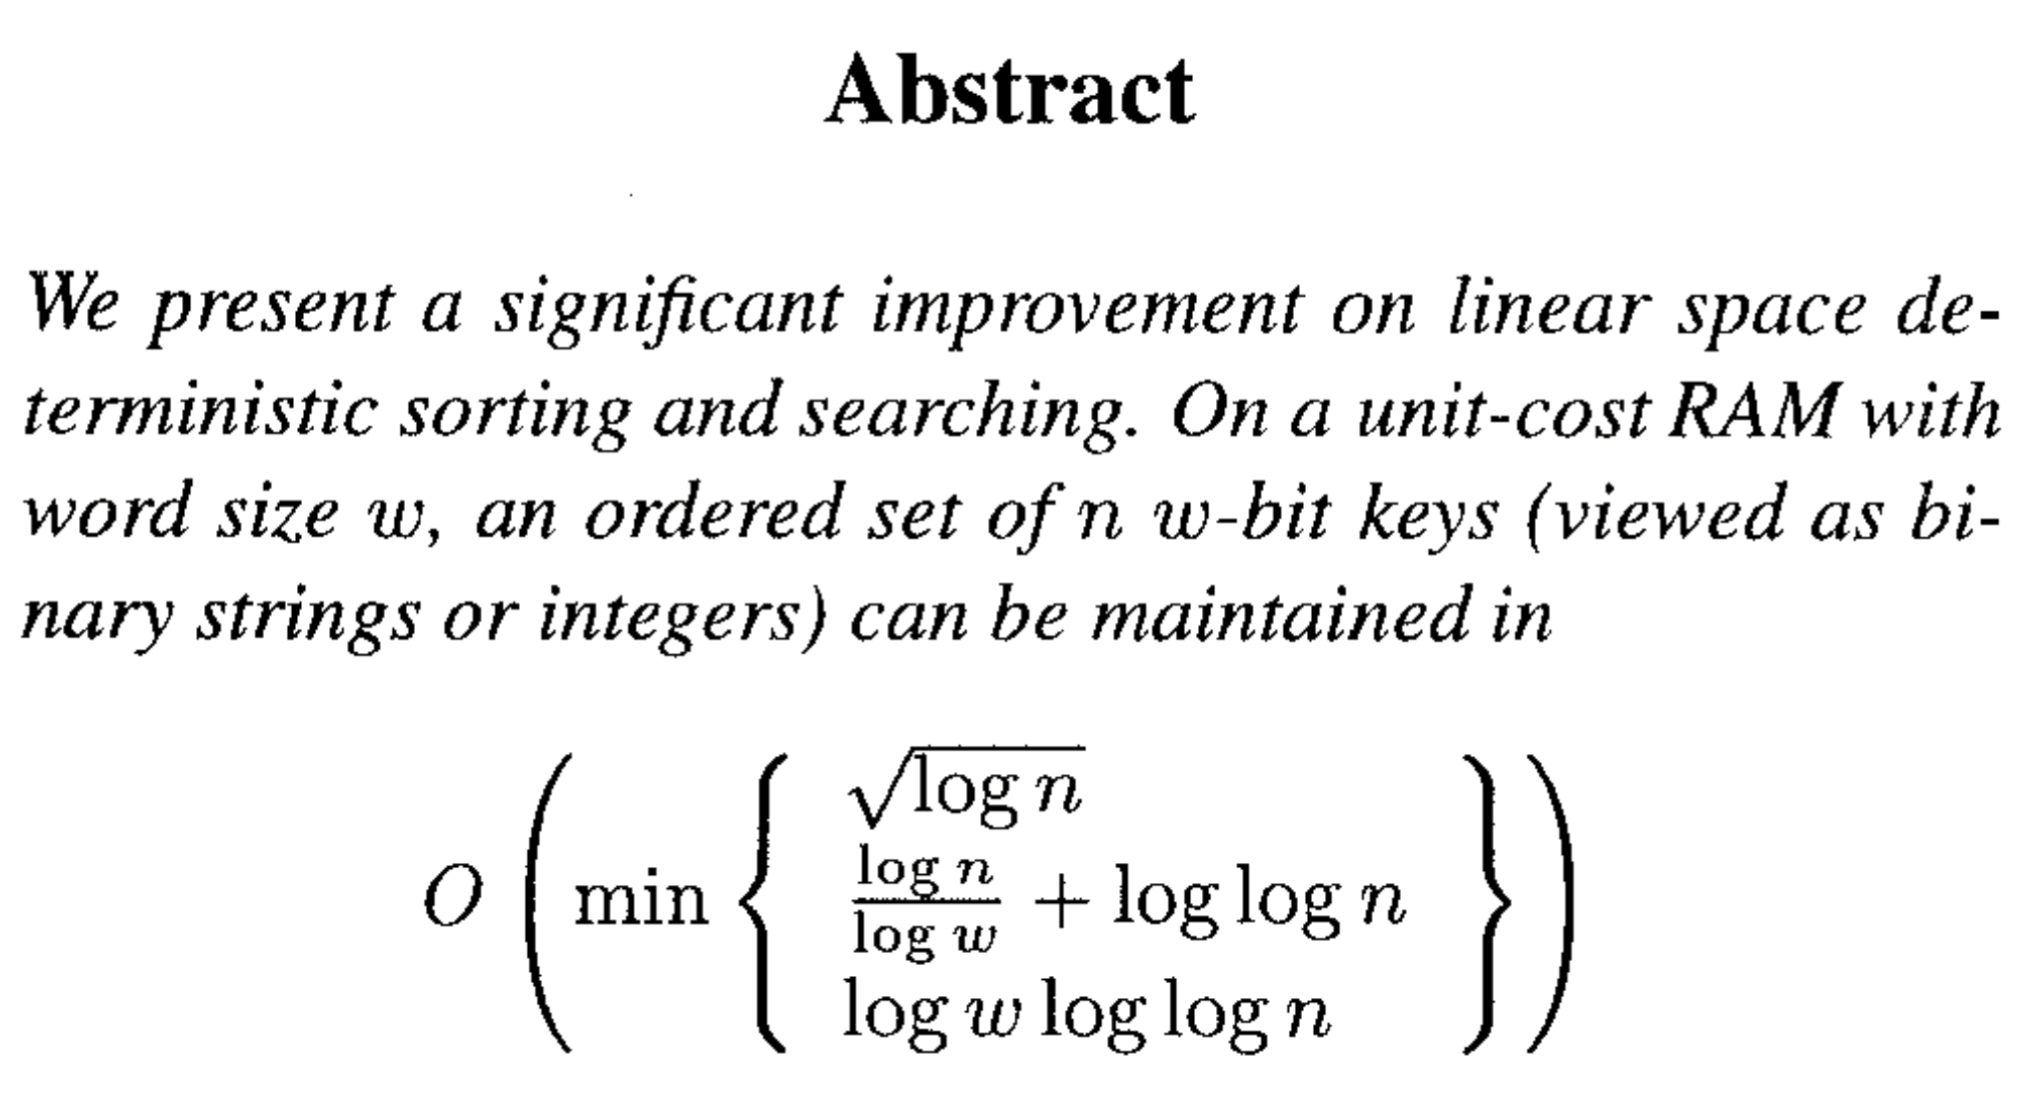
\includegraphics[scale=0.1]{slides/alphabet_trees/exponential_tree_abstract.png}
         \end{center}
    \end{column}
    \end{columns}
}